\usetikzlibrary{arrows.meta,positioning}

\tikzset{
loopnode/.style={
  draw=black!75,
  thick,
  rounded corners=2pt,
  fill=blue!6,
  align=center,
  font=\footnotesize,
  minimum width=2.85cm,
  minimum height=8mm
},
looparrow/.style={
  -{Latex[length=2.5mm,width=2mm]},
  thick,
  draw=black!75
}
}

\begin{figure}[!tbp]
\centering
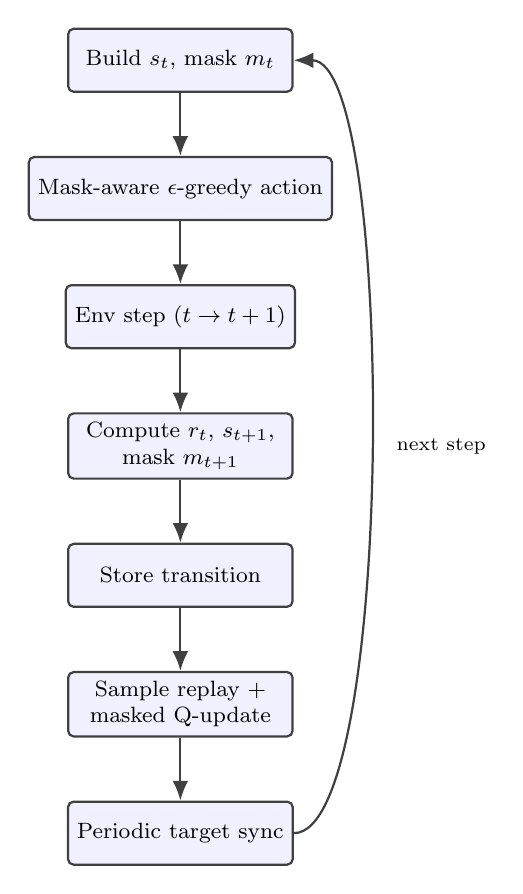
\begin{tikzpicture}[node distance=8mm and 5mm]

\node[loopnode] (obs) {Build $s_t$, mask $m_t$};
\node[loopnode, below=of obs] (act) {Mask-aware $\epsilon$-greedy action};
\node[loopnode, below=of act] (step) {Env step ($t \to t+1$)};
\node[loopnode, below=of step] (next) {Compute $r_t$, $s_{t+1}$,\\mask $m_{t+1}$};
\node[loopnode, below=of next] (store) {Store transition};
\node[loopnode, below=of store] (learn) {Sample replay +\\masked Q-update};
\node[loopnode, below=of learn] (sync) {Periodic target sync};

\draw[looparrow] (obs) -- (act);
\draw[looparrow] (act) -- (step);
\draw[looparrow] (step) -- (next);
\draw[looparrow] (next) -- (store);
\draw[looparrow] (store) -- (learn);
\draw[looparrow] (learn) -- (sync);
\draw[looparrow] (sync.east) .. controls +(1.3,0) and +(1.3,0) .. node[midway,right=2mm,font=\scriptsize]{next step} (obs.east);

\end{tikzpicture}
\caption{Training-loop schematic with mask-aware interaction, complete transition construction, replay learning, and periodic target synchronization.}
\label{fig:training_loop}
\end{figure}
